%% ==============================
\chapter{\iflanguage{ngerman}{Implementierung}{Implementation}}
\label{sec:implementation}
%% ==============================




Nachdem im letzten Kapitel das Softwaredesign besprochen wurde, beschäftigt sich das Kommende mit der Implementierung an sich.


Es ergaben sich bei der Implementierung verschiedene Probleme. Beispielsweise wurde anfangs das Verfahren mit MRT-Daten getestet. Dies war von wenig Erfolg, da die Volumendaten große Unterschiede zu den CT-Daten aufweisen und somit das Verfahren nicht funktionierte.


Die vorgestellten Module erben alle von der abstrakten \textit{BaseModule} Klasse, die es ihnen vorschreibt, eine \textit{Call} sowie eine \textit{PrintHelp} Methode zu implementieren.
\newline
Ruft der Benutzer ein Modul des Helpers über den jeweiligen Befehl in der Konsole auf, so wird die jeweilige \textit{Call} Methode, mit denen vom Benutzer gegebenen Parameter, ausgeführt.
\newline
Es existiert für jeden der Berechnungsschritte der Gradienten, LH-Werte, LH-Cluster und Räumlichen-Cluster eine eigene statische Klasse, die eine öffentliche Methode besitzt. Diese berechnet für die gegebenen Parameter den jeweiligen Schritt und gibt das Ergebnis zurück. 
\newline
Beispielsweise wird in der \textit{Call} Methode des \textit{LHHistogram} Moduls, zuerst die \textit{CalcGradientVolume} Funktion der \textit{Gradient} Klasse mit dem Intensitätsvolumen als Parameter aufgerufen. Danach wird die \textit{LHValuesVolume} Methode der \textit{LHValues} Klasse mit dem Ergebnis der vorherigen Funktion als Parameter ausgeführt. Aus dessen Ergebnis wird in der \textit{Call} Methode des Moduls direkt das LH-Histogramm erstellt und gespeichert. Im Modul \textit{ClusterVolume} läuft die Berechnung ebenso über das Aufrufen von den Methoden der jeweiligen Klassen ab.
\newline
Das Modul \textit{MergeCluster} führt seine Berechnung komplett in der \textit{Call} Funktion, da die Kalkulation nicht sehr aufwändig ist, aus.
\newline
Die Implementierung der Klassen und deren Methoden ist das Thema dieses Kapitels und wird im Folgenden genauer erläutert.
\newline
Bei der  Kalkulation der Gradienten wird parallel über jeden Voxel im Intensitätsvolumen iteriert und für jeden die Implementierung von Hong's Methode \cite{} aufgerufen.
\newline
Für die Berechnung der Methode wird eine Gewichtung und die Koordinaten aller 64 Punkte im Koordinatensystem der lokalen Nachbarschaft benötigt. Da das gesamte Volumen die selbe Voxellänge hat und die Koordinaten in der lokalen Nachbarschaft immer gleich sind, können diese beiden Werte für alle 64 Nachbarn einmalig in einem Vorverarbeitungsschritt berechnet werden. Sie werden dabei in einem 64 Elemente großes Array, mit der gleichen Nummerierung wie in \autoref{fig:nachbarschaft} gezeigt, gespeichert. Bei der Kalkulation jedes Gradienten müssen lediglich die beiden Arrays durch iteriert werden um die entsprechenden Gewichtung und Koordinate  des Nachbars zu erhalten


\begin{figure}[!h] 
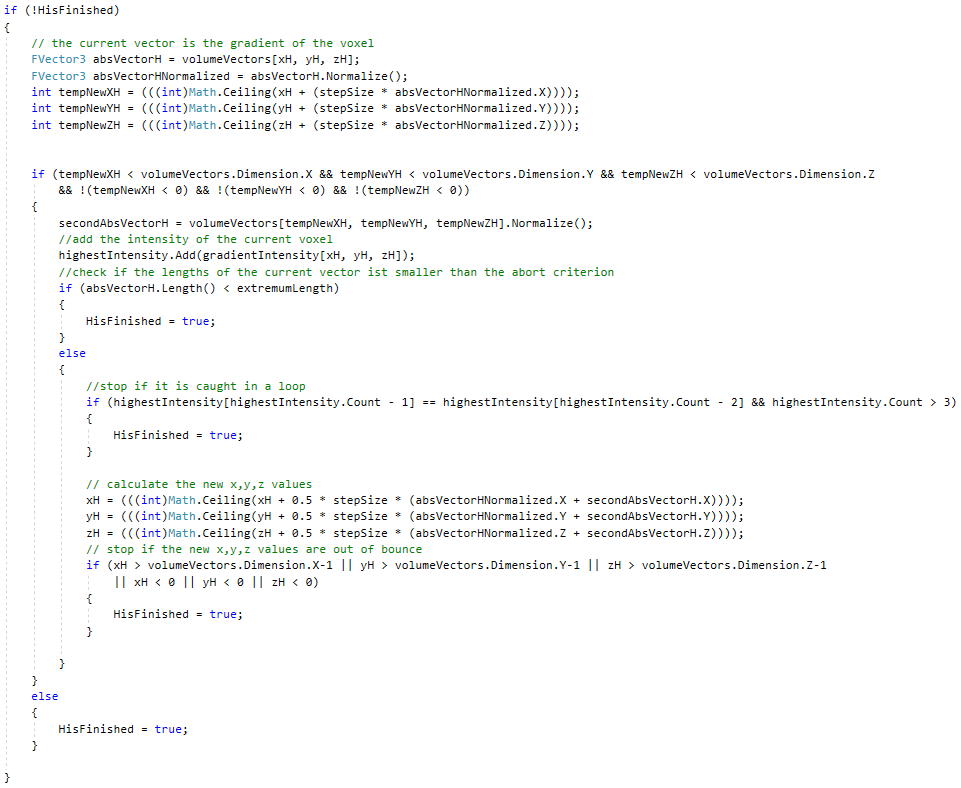
\includegraphics[width=1.2\textwidth]{Logos/LH_Code.PNG}
\caption{Implementierung der Berechnung der High-Werte} 
\label{fig:lh_code} 
\end{figure}


In \autoref{fig:lh_code} kann man den Code zur Berechnung der High-Werte sehen. Der Code liegt innerhalb einer while-Schleife, die so lange aufgerufen wird, bis die Berechnung des Low- und des High-Wertes abgeschlossen, also \textit{LisFinished} und \textit{HisFinished} true sind. Die Berechnung des Low-Wertes ist ebenfalls in der Schleife und sieht bis auf die Richtung der neuen \textit{absVector} und \textit{secondAbsVector} gleich aus. Folglich sind alle hier gegebenen Erklärung und Anmerkungen ebenso auf die Berechnung der Low-Werte zu beziehen.
\newline
Am Anfang eines Durchlaufes wird der normalisierte Gradienten des aktuellen Punktes in \textit{absVectorNormalized} gespeichert. Anschließend wird der Punkt des zweiten normalisierten Vektors berechnet. Liegt dieser außerhalb des Volumens, so wird die Integration beendet. Liegt er jedoch innerhalb des Volumens, so wird der \textit{secondAbsVector} ausgelesen und der Intensitätswert des aktuellen Punktes zu der Liste \textit{highestIntensity} hinzugefügt. Ist der Gradient des aktuellen Punktes kleiner als die \textit{extremumLength}, welche im Falle von CT-Daten bei null liegt, wird die Integration beendet.
\newline
Andernfalls wird zunächst mithilfe der \textit{highestIntensity} Liste nach Schleifen gesucht. Bei sehr kleinen Gradienten, die jedoch größer als null sind, kann es vorkommen, dass das Verfahren immer wieder den selben Punkt findet und somit in einer Endlosschleife feststeckt. Wie in \autoref{fig:lh_code]} zu sehen ist, wird dabei jedoch erst getestet ob die Liste schon mehr als 3 Einträge hat. Dies geschieht aus dem Grund, dass anfangs, vor der while-Schleife bereits der Intensitätswert des Startvoxels zur Liste hinzugefügt werden muss. Dies geschieht aus dem Grund, dass sonst, würde das Verfahren bei dem ersten Abbruchkriterium bei der ersten Iteration schon stoppen, die \textit{highestIntensity} Liste leer wäre, und es kein Ergebnis für den High-Wert gäbe. Diese Kontrolle könnte jedoch über die Koordinaten der iterierten Punkte geschehen, um dem unwahrscheinlichem Fall, dass zwei durch die Integration hintereinander besuchte Punkte genau den selben Intensitätswert haben.
\newline
Anschließend wird der nächste Punkt der Integration mithilfe von \textit{absVectorNormalized} und \textit{secondAbsVecotr} gemäß Heun's Methode, die im Kapitel der Methode vorgestellt wurde, ermittelt. Erneut endet die Integration, falls der neu berechnete Punkt außerhalb des Volumens liegt.
\newline
Dieser Vorgang wiederholt sich für den High- als auch für den Low-Wert solange, bis die Integration aus einem der gegebenen Abbruchkriterien stoppt. In diesem Fall wird der letzte Eintrag der \textit{highestIntensity} Liste ausgelesen und als Ergebnis für den High-Wert gespeichert. Ebenso passiert dies mit der für die Low-Werte äquivalenten \textit{lowestIntensity} Liste.
\newline
Der Fall, dass ein Iterationsschritt in einer der gezeigten Formen außerhalb des Volumens liegt, und deshalb das Verfahren gestoppt wird, kommt in ungefähr 2-\%-3\% der Fälle vor. Des Weiteren kommt es bei zirka 25\% aller Berechnung dazu, dass die LH-Werte vertauscht waren, also der Low- größer als der High-Wert war. Dem wird entgegengewirkt, indem bei einem Vorkommen dieses Problems die beiden Werte vertauscht gespeichert werden. Es war noch nicht möglich den Grund für diese Verwechslung herauszufinden.


Die Implementierung des LH-Clusterings wurde mit einer parallelen for-Schleife realisiert, die über die L-Werte mit der Schrittweite von 5 iteriert. Für jede Spalte i wird dann die in \autoref{alg:clustering} beschriebene Funktion aufgerufen.
\newline
Die erste for-Schleife iteriert über die H-Werte. Der Parameter j beginnt mit dem Wert i und wird, wie dieser, mit der Schrittweite 5 hochgezählt. Dies hat den Grund, dass es im LH-Histogramm keine Einträge gibt, bei denen der Low- höher als der High-Wert ist. Alle durch die beiden Schleifen entstehenden Punkte $(i, j)$ sind jeweils die Startpunkte einer Clustersuche.
\newline
Um nicht zu viele Cluster zwischenspeichern zu müssen und erst ganz am Ende alle ähnlichen Cluster zu verschmelzen, werden bereits am Ende jeder Spalte deren Ergebniscluster soweit wie möglich verschmolzen.
\newline
Weiterhin speichert der temporäre Cluster \textit{AktuellerCluster} lediglich die Koordinaten der zum Cluster dazugehörigen Punkte im Histogramm, jedoch nicht die räumlichen Informationen der darin gespeicherten Voxel, ab. Erst am Ende der parallelen Schleife, wenn alle Ergebnisse gesammelt und die Cluster verschmolzen wurden, werden diese Daten ausgelesen. Dies spart Speicherplatz und Berechnungszeit, da in einem einzigen Kästchen im LH-Histogramm mehrere Tausend Voxel gespeichert sein können.


\IncMargin{1em}
\begin{algorithm}
\SetKwData{Left}{left}\SetKwData{This}{this}\SetKwData{Up}{up}
\SetKwFunction{Union}{Union}\SetKwFunction{FindCompress}{FindCompress}
\SetKwInOut{Input}{input}\SetKwInOut{Output}{output}

 \Input{LH-Histogramm, Spalte i}
 \Output{LH-Clusters}
 \BlankLine
 $AlleErgbnisCluster$\;
 $Mittelpunkt$\;
 $AlterMittelpunkt$\;
 $AktuellerCluster$\;
 \For{$j\leftarrow i$ \KwTo Rand des Histogramms, Schrittweite: 5}{
  $Mittelpunkt \leftarrow (i,j)$\;
 \While{Abstand(NeuerMittelpunkt, AlterMittelpunkt) > Threshold * Bandweite}{
  \For{$(k, l)\leftarrow$ Alle Punkte im Radius der Bandweite um den Mittelpunkt}{
      \If{NochNichtTeilDesClusters((k, l))}{
	$AktuellerCluster.Hinzufuegen((k, l))$\;
     }
    }
   $AlterMittelpunkt \leftarrow Mittelpunkt$\;
    $Mittelpunkt \leftarrow NeuenMittelpunktBerechnen(AktuellerCluster)$\;
  }
  $AlleErgebnisCluster.Hinzufügen(AktuellerCluster)$\;
 $ Leeren(AktuellerCluster)$\;
 }
$VerschmelzeNaheCluster(AlleErgebnisCluster)$\;
$return$ $AlleErgebnisCluste$r\;

 \caption{Pseudocode der Implementierung der LH-Cluster}
 \label{alg:clustering}
\end{algorithm}\DecMargin{1em}


Das LH-Clustering wurde anfangs wie im Paper von Nguyen \cite{nguyen2012clustering} über das gesamte Histogramm mit einer Bandweite von 7\% des maximalen LH-Wertes für jeden Kasten berechnet. Dies ist aus mehreren Gründen schlecht. Zum einen ist der maximale LH-Wert sehr hoch, über 4000, obwohl in etwa nur 0,3\% Voxel einen Wert von über 2400 haben. Zum anderen liegen über 5\% der LH-Werte unter 5. Die Kombination aus diesen Gründen, machte das Clustering extrem langsam. Im Bereich von 0 bis 50  wurde in einem sehr großen Radius geclustert, wodurch mit jeder Iteration sehe viele Cluster gefunden und hinzugefügt werden mussten.
\newline
Eine erste Maßnahme um das Problem zu beheben, war es alle Low- und High- Werten, die über 2400 waren jeweils auf 2400 zu setzten. Dadurch wurden nur wenige Werte verändert und der Clusteringradius wurde deutlich kleiner. Dies konnte das beschriebene Problem jedoch nicht alleine lösen, da immer noch viele Punkte gefunden und dies für jeden Kasten im Histogramm durchgeführt werden musste.
\newline
Also wurde als nächste Verbesserung eine Schrittweite beim Clustern eingeführt. Dies geschah aus der Beobachtung heraus, dass zwei bis drei oder eventuell sogar mehr direkt nebeneinanderliegende Kasten meist zum selben oder einen so ähnlichen Cluster führen, dass diese im letzten Schritt des Clusteringsverfahrens verschmolzen wurden. Diese Änderung verbesserte die Berechnungszeit erneut, jedoch  dauert die Berechnung immer noch relativ lange und es entstanden sehr viele Cluster. Diese durchzuschauen benötigte viel Zeit und das Gehirn wurde dabei meist als viele sehr große Cluster erkannt. Daraufhin wurde das Clustering auf einen LH-Wertbereich von 1025 bis 1075 begrenzt und die Bandweite auf 0,1\% des maximalen LH-Wertes gesetzt. Diese Änderung führte zum Erfolg und das Ventrikelsystem war innerhalb der paar hunderten Clustern mit ein bisschen Aufwand zu erkennen.
\newline
In der statischen Klasse \textit{SpatialClustering} ist die Implementierung zur Berechnung der räumlichen Cluster und dem Clustervolumen der IDs zu finden.
\newline
Die Kalkulation der räumlichen Clustern wurde dabei, wie die Berechnung der LH-Cluster, mit einer parallelen for-Schleife realisiert. Diese iteriert über die LH-Cluster und ruft für jeden Cluster die in \autoref{fig:spatclust_code} gezeigte Funktion auf. Die Cluster sind in der globalen Liste \textit{LHClusters} gespeichert. Sie haben den Typ einer Liste von \textit{IVector3}. 
\newline
Die Suche nach Clustern liegt in einer while-Schleife, die so lange ausgeführt wird, solange der LH-Cluster genug Elemente hat, damit ein Cluster mit der Mindestgröße an Elementen gefunden werden kann. 
\newline
Das Finden von Clustern läuft dabei folgendermaßen ab. Der erste Punkt im LH-Cluster wird als Startmittelpunkt gewählt. Danach wird durch alle Punkte iteriert und diejenigen die innerhalb der Bandweite liegen sowohl zum temporärem Cluster \textit{currentSpatialCluster} als auch zum HashSet der zu entfernenden Punkte \textit{toRemove} hinzugefügt. Anschließend werden, alle Elemente von \textit{toRemove} aus dem LH-Cluster entfernt und wie beim LH-Clustering auch ein neuer Mittelpunkt errechnet. Wenn das Abbruchkriterium der zwei naheliegenden aufeinanderfolgenden Mittelpunkte erfüllt ist, wird der temporäre Cluster \textit{currentSpatialCluster} zur Liste der Ergebniscluster \textit{resultClusters} hinzugefügt, falls er genug Elemente besitzt.
\newline
Für die Bandweite und die minimale Distanz für das Abbruchkriterium wurden im Paper von Nguyen \cite{} keine Werte angegeben. In dieser Bachelorarbeit wurde die Bandweite auf 15 und die Distanz auf 0,01 gesetzt. Diese Werte wurden durch Testen herausgefunden und führten zu den besten Ergebnissen.
\newline
Anschließend wird in der Funktion \textit{ComputeIDs}, der die Cluster als Parameter übergeben werden, das Clustervolumen erstellt und zurückgegeben.



\begin{figure}[!h] 
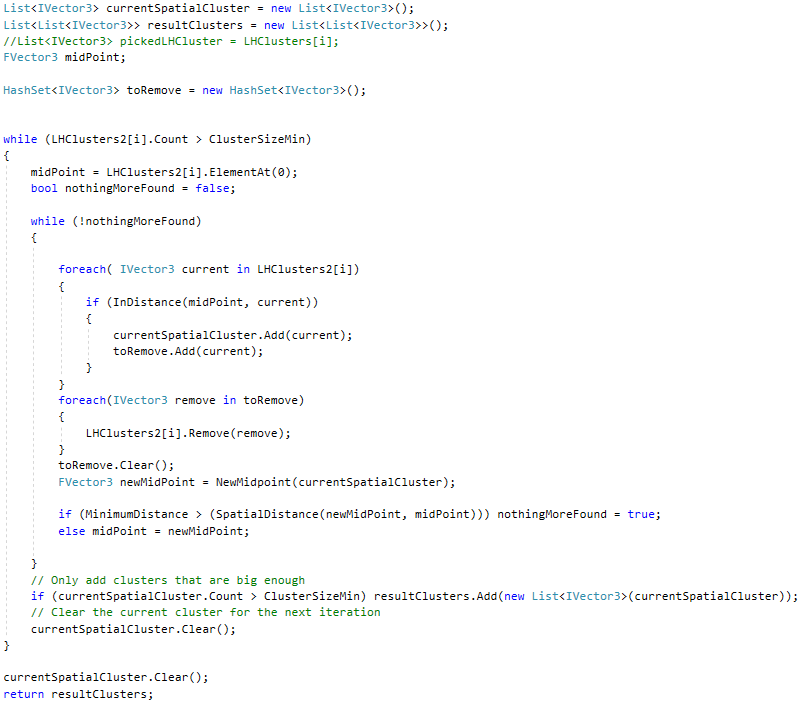
\includegraphics[width=1.2\textwidth]{Logos/Spatial_Code.PNG}
\caption{Implementierung der Berechnung der Gewichte und Koordinaten} 
\label{fig:spatclust_code} 
\end{figure}


Die Erweiterung die am Renderer vorgenommen wurden, wurden im Shader programmiert. Zuerst wurde eine drop-down-list hinzugefügt, über die der Nutzer zwischen den Modi \textit{Default}, \textit{SpecificValue} und \textit{SpecificValueRange} wählen konnte. Weiterhin wurden drei Textfelder hinzugefügt, über die es dem Anwender möglich ist den spezifischen Wert als auch den Wertebereich anzugeben. Des Weiteren wurde noch ein Farbfeld hinzugefügt, mit welchem die Farbe, in der hervorgehobenen Bereiche dargestellt wird, anzeigt wird und vom Benutzer verändert werden kann.
\newline
Der \textit{Default} Modus steht hierbei für die schon vorher dagewesene Implementierung der Farbgebung. Diese wurde weitestgehend in den beiden anderen beiden Modi übernommen. Der Unterschied besteht jedoch darin, dass wenn ein Voxel bei \textit{SpeicifcValue}mit dem spezifischen Wert, oder bei \textit{SpecificValueRange} innerhalb des Wertebereichs gefunden wird, dieser in der Farbe des Farbfeldes angezeigt wird. Alle andern Voxel bekommen die selbe Farbe, die sie auch im \textit{Default} Modus erhalten würden.























































